\section{pbdR}
\makesubcontentsslides

\subsection{The pbdR Project}
\makesubcontentsslidessec

\begin{frame}{\pbdR Interfaces to Libraries: Sustainable Path}
  \vspace{-1ex}
  \centering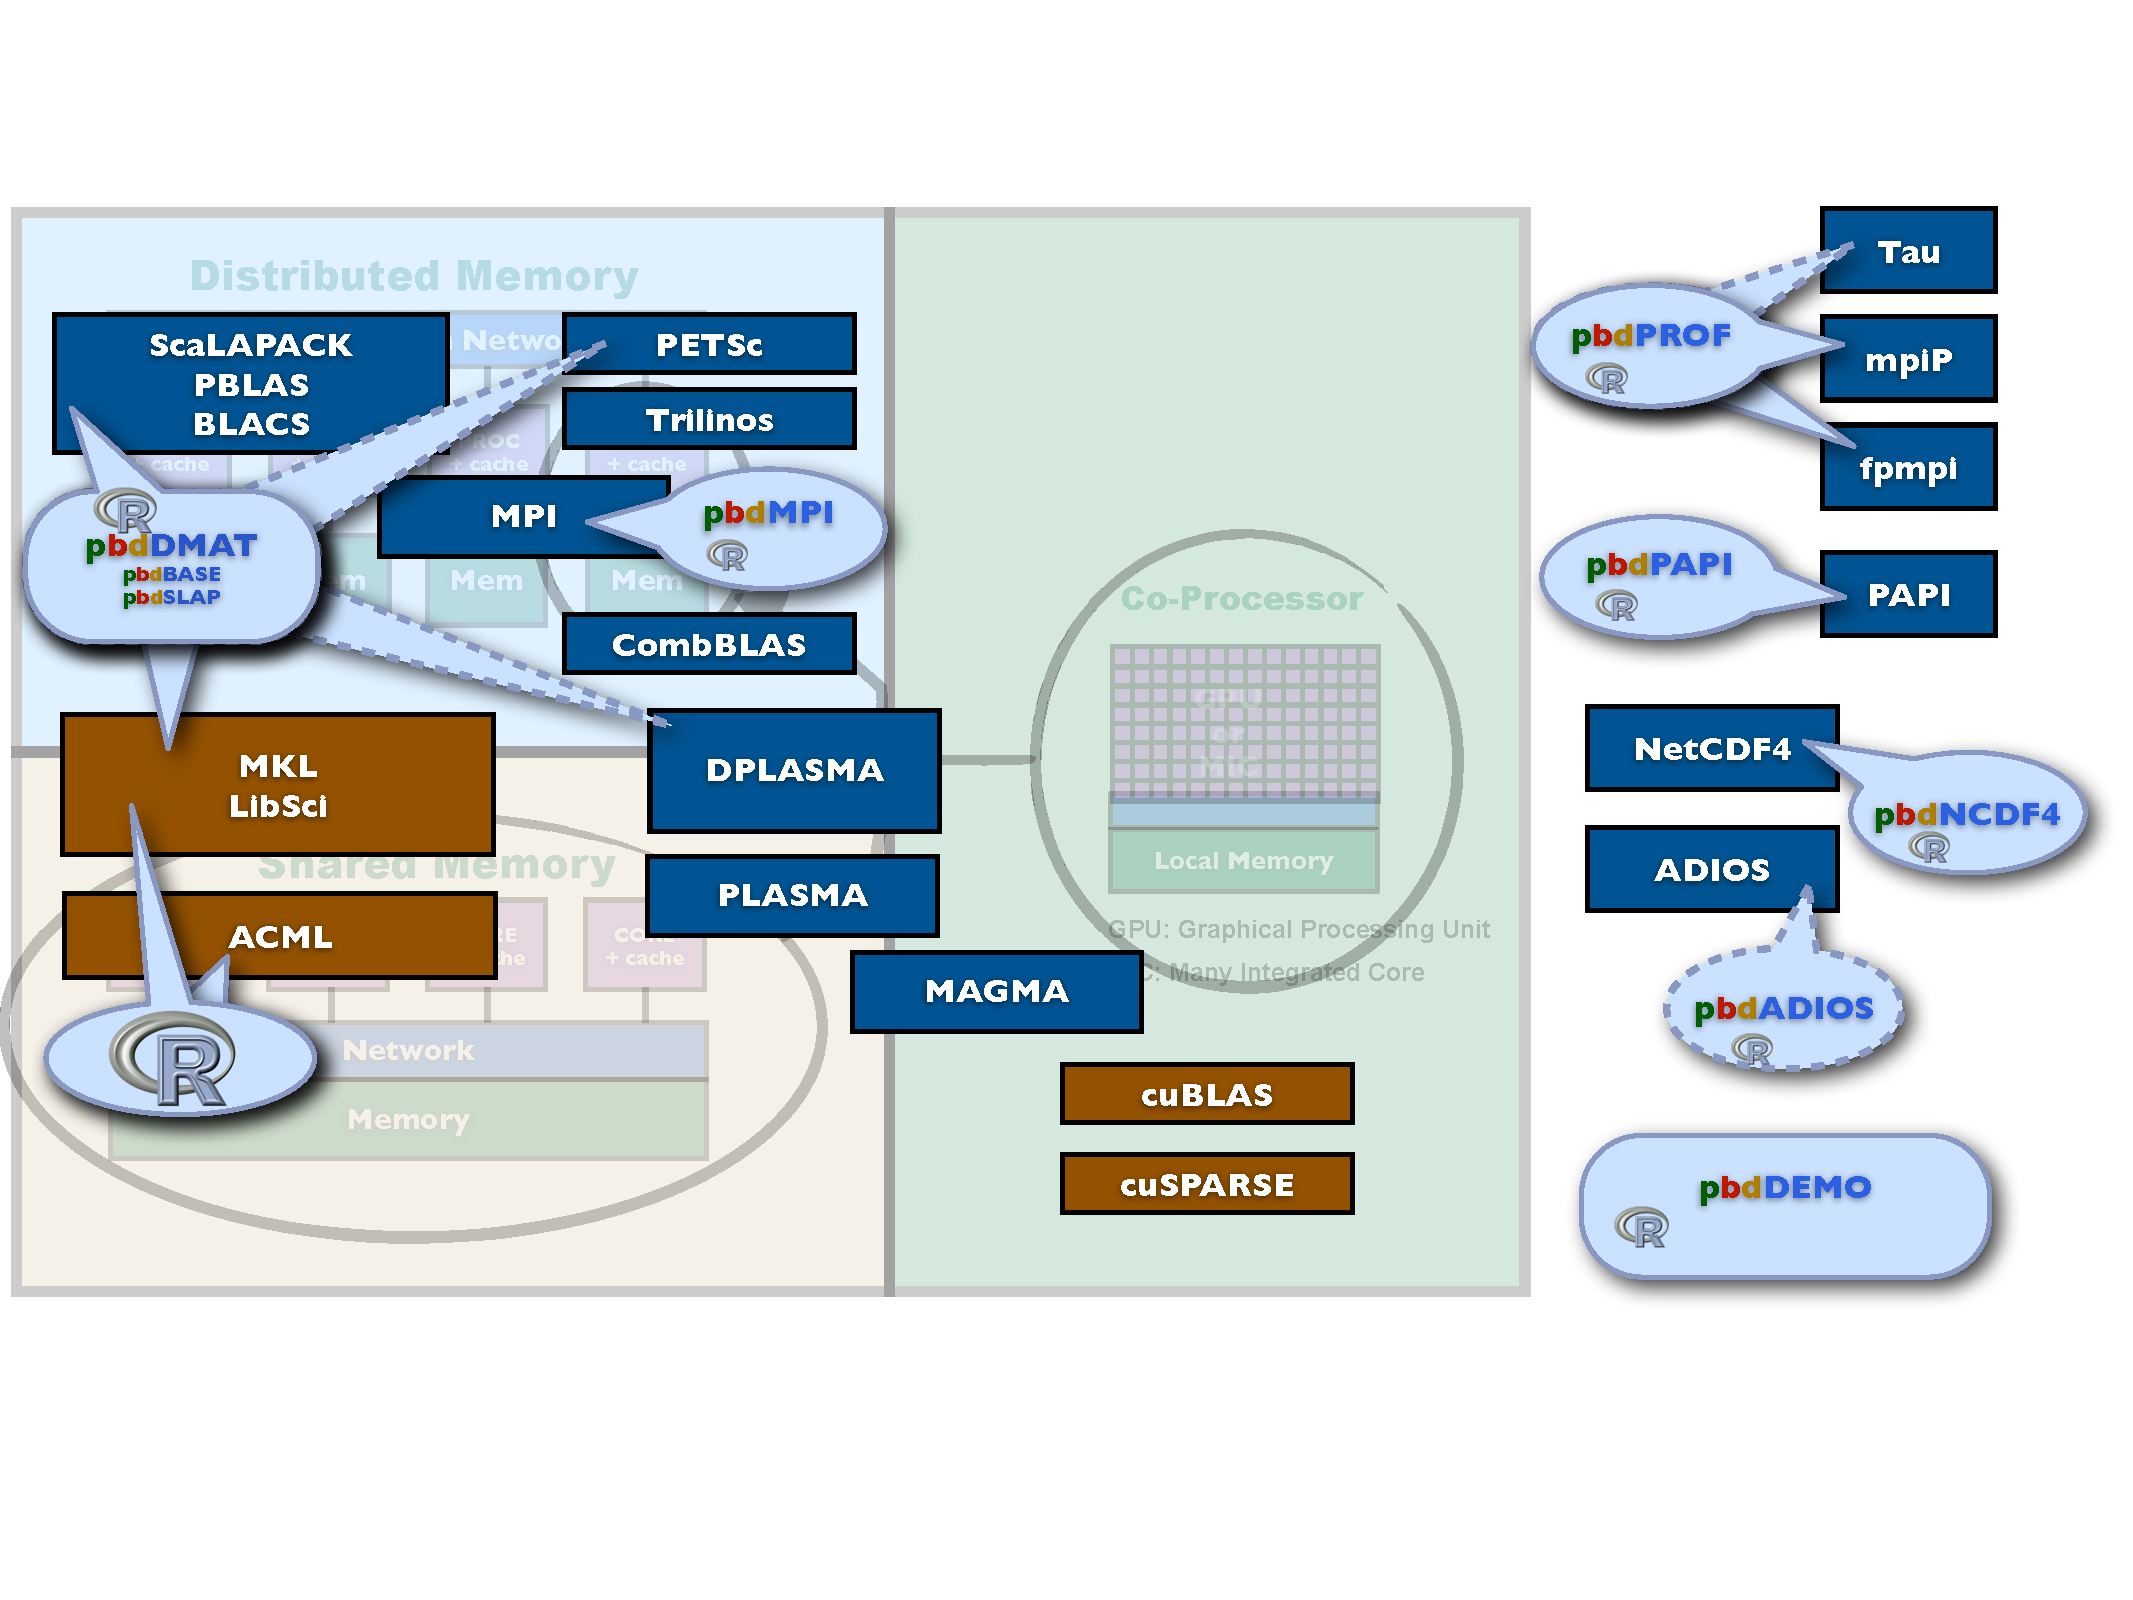
\includegraphics[trim=0cm 5cm 0cm 3cm,clip=true,width=0.85\textwidth]
  {../common/pics/hardware/ParallelHardware27.pdf}
  \scriptsize
  \begin{block}{Why use HPC libraries?}
    \begin{itemize}[<+-|alert@+>]
    \item The HPC community is 30 years beyond ``embarrassingly parallel.''
    \item \emph{They're tested.} \emph{They're
        fast.}  \emph{They're scalable.}
    \item Many science communities are invested in their API.
    \item Data analysis uses much of the same math as simulation science.
    \end{itemize}
  \end{block}
\end{frame}

\subsection{pbdMPI}
\makesubcontentsslidessec

\begin{frame}
  \begin{block}{pbdMPI: a High Level Interface to MPI}
    \begin{itemize}
    \item API is simplified: defaults in control objects.
    \item S4 methods: extensible to complex \R objects.
    \item Additional error checking
    \item Array and matrix methods without serialization: faster than
      \pkg{Rmpi}.
    \end{itemize}
    \begin{center}
      \vspace{0.2cm}\scriptsize
      \begin{tabular}{ll} \hline\hline
        \pkg{pbdMPI} (S4) & \pkg{Rmpi}                \\ \hline
        \code{\color{blue}allreduce}    & \code{mpi.allreduce}      \\
        \code{\color{blue}allgather}    & \code{mpi.allgather},
        \code{mpi.allgatherv},
        \code{mpi.allgather.Robj} \\
        \code{bcast}        & \code{mpi.bcast},
        \code{mpi.bcast.Robj}     \\
        \code{gather}       & \code{mpi.gather},
        \code{mpi.gatherv},
        \code{mpi.gather.Robj}    \\
        \code{recv}         & \code{mpi.recv},
        \code{mpi.recv.Robj}      \\
        \code{reduce}       & \code{mpi.reduce}         \\
        \code{scatter}      & \code{mpi.scatter},
        \code{mpi.scatterv},
        \code{mpi.scatter.Robj}   \\
        \code{send}         & \code{mpi.send},
        \code{mpi.send.Robj}      \\ \hline \hline
      \end{tabular}
    \end{center}
  \end{block}
\end{frame}

\begin{frame}[fragile]
  \begin{block}{Integer?\qquad Not always obvious in R.}
    \vspace{-.2cm}
    \begin{lstlisting}
> is.integer(1)
[1] FALSE
> is.integer(2)
[1] FALSE
> is.integer(1:2)
[1] TRUE
    \end{lstlisting}
  \end{block}
  \begin{block}{Often it's best to let the machine figure it out}\pause
    \begin{minipage}[t]{.475\textwidth}
      \begin{lstlisting}[title=Rmpi]
# int
mpi.allreduce(x, type=1)
# double
mpi.allreduce(x, type=2)
      \end{lstlisting}
    \end{minipage}
    \hfill
    \begin{minipage}[t]{.475\textwidth}
      \begin{lstlisting}[title=pbdMPI]
allreduce(x)
      \end{lstlisting}
      % \vspace{1em}
      % \hspace{1em}{\small S4. Batch only! (No spawning)}
    \end{minipage}
  \end{block}
\end{frame}



% \begin{frame}[fragile,shrink]
%   \begin{block}{Embarrassingly Parallel Computation}\pause
%     \vspace{-1ex}
%     \begin{minipage}[t]{.45\textwidth}
%       \begin{lstlisting}[title=EPforeach.R "asking for parallel",basicstyle=\tiny]
% library(doMPI, quiet=TRUE)
% cl <- startMPIcluster()
% registerDoMPI(cl)

% n <- 10
% myIn <- vector("list", n)

% myFun <- function(x) {
%   s <- sum(rnorm(10000))
%   rank <- mpi.comm.rank(comm=0)
%   return(paste(s, "from", rank))
% }

% results <- foreach(i = 1:n) %dopar% {
%   out <- myFun(myIn[[i]])
% }

% print(results)

% closeCluster(cl)
% mpi.quit()
%       \end{lstlisting}
%     \end{minipage}
%     \hfill
%     \begin{minipage}[t]{.5\textwidth}
%       \begin{lstlisting}[title=EPpbdR.R "thinking parallel",basicstyle=\tiny]
% library(pbdMPI, quiet=TRUE)
% init()

% myChunk <- get.jid(n <- 10)
% myIn <- vector("list", length(myChunk))
% myOut <- vector("list", length(myChunk))

% myFun = function(x) {
%   s <- sum(rnorm(10000))
%   rank <- comm.rank()
%   return(paste(s, "from", rank))
% }

% for(i in 1:length(myChunk)) {
%   myOut[[i]] <- myFun(myIn[[i]])
% }
% results <- gather(myOut)

% comm.print(results)
% finalize()
%       \end{lstlisting}
%     \end{minipage}
%   \end{block}
% \end{frame}


\begin{frame}[fragile]{SPMD Runs Many Copies of One Code}
  \begin{exampleblock}{SPMD Hello World: a ``map-reduce'' to all}
    \vspace{-1.5ex}
    \centering
    \begin{lstlisting}[title=map-reduce.r]
library(pbdMPI, quiet = TRUE)
init()

## Your "Map" code
n <- comm.rank() + 1

## Now "Reduce" but give the result to all
all_sum <- allreduce(n) # Sum is default

text <- paste("Hello: n is", n, "sum is", all_sum )
comm.print(text, all.rank=TRUE)

finalize()
    \end{lstlisting}
    \vspace{-4.5ex}
    \begin{columns}[t,onlytextwidth]
      \begin{column}{0.54\textwidth}
        \begin{lstlisting}[backgroundcolor=\color{white},keywordstyle=\color{black},
title=Execute this batch script via:]
mpirun -np 2 Rscript map-reduce.r
        \end{lstlisting}
      \end{column}
      \hfill
      \begin{column}{0.46\textwidth}
        \begin{lstlisting}[title=Output:]
COMM.RANK = 0
[1] "Hello: n is 1 sum is 3"
COMM.RANK = 1
[1] "Hello: n is 2 sum is 3"
        \end{lstlisting}
      \end{column}
    \end{columns}
  \end{exampleblock}
\end{frame}

\subsection{pbdDMAT}
\makesubcontentsslidessec

\begin{frame}{Dense Matrix and Vector Operations}
  \begin{block}{A matrix is mapped to a processor grid shape}
    \begin{table}[ht]
      \centering
      % \begin{subfigure}[b]{0.23\textwidth}
      %   \centering
      %   $\left[\begin{tabular}{l}
      %       0 \\ 1 \\ 2 \\ 3 \\ 4 \\ 5
      %     \end{tabular}\right]^T$
      %   \caption{$1\times 6$}
      % \end{subfigure}
      \begin{subfigure}[b]{0.23\textwidth}
        \centering
        $\left[\begin{tabular}{llllll}
            0 & 1 & 2 & 3 & 4 & 5
          \end{tabular}\right]$
        \vspace{1.5cm}
        \caption{$1\times 6$}
      \end{subfigure}%\hspace{-1cm}
      \begin{subfigure}[b]{0.23\textwidth}
        \centering
        $\left[\begin{tabular}{lll}
            0 & 1 & 2\\
            3 & 4 & 5
          \end{tabular}\right]$
        \caption{$2\times 3$}
      \end{subfigure}%
      \begin{subfigure}[b]{0.23\textwidth}
        \centering
        $\left[\begin{tabular}{ll}
            0 & 1 \\
            2 & 3\\
            4 & 5
          \end{tabular}\right]$
        \caption{$3\times 2$}
      \end{subfigure}
      \begin{subfigure}[b]{0.23\textwidth}
        \centering
        $\left[\begin{tabular}{l}
            0 \\ 1 \\ 2 \\ 3 \\ 4 \\ 5
          \end{tabular}\right]$
        \caption{$6\times 1$}
      \end{subfigure}
      \caption{Processor Grid Shapes with 6 Processors}\label{fig:gridshapes}
    \end{table}
  \end{block}
\end{frame}

\begin{frame}[shrink]
\begin{exampleblock}{2$\times$3 block-cyclic grid on 6 processors:
    Global view ``ddmatrix'' class}
\begin{align*}
x &= \left[
      \begin{array}{ll|ll|ll|ll|l}
      \color{g11}x_{11} & \color{g11}x_{12} & \color{g12}x_{13} & \color{g12}x_{14} & \color{g13}x_{15} & \color{g13}x_{16} & \color{g11}x_{17} & \color{g11}x_{18} & \color{g12}x_{19}\\
      \color{g11}x_{21} & \color{g11}x_{22} & \color{g12}x_{23} & \color{g12}x_{24} & \color{g13}x_{25} & \color{g13}x_{26} & \color{g11}x_{27} & \color{g11}x_{28} & \color{g12}x_{29}\\\hline
      \color{g21}x_{31} & \color{g21}x_{32} & \color{g22}x_{33} & \color{g22}x_{34} & \color{g23}x_{35} & \color{g23}x_{36} & \color{g21}x_{37} & \color{g21}x_{38} & \color{g22}x_{39}\\
      \color{g21}x_{41} & \color{g21}x_{42} & \color{g22}x_{43} & \color{g22}x_{44} & \color{g23}x_{45} & \color{g23}x_{46} & \color{g21}x_{47} & \color{g21}x_{48} & \color{g22}x_{49}\\\hline
      \color{g11}x_{51} & \color{g11}x_{52} & \color{g12}x_{53} & \color{g12}x_{54} & \color{g13}x_{55} & \color{g13}x_{56} & \color{g11}x_{57} & \color{g11}x_{58} & \color{g12}x_{59}\\
      \color{g11}x_{61} & \color{g11}x_{62} & \color{g12}x_{63} & \color{g12}x_{64} & \color{g13}x_{65} & \color{g13}x_{66} & \color{g11}x_{67} & \color{g11}x_{68} & \color{g12}x_{69}\\\hline
      \color{g21}x_{71} & \color{g21}x_{72} & \color{g22}x_{73} & \color{g22}x_{74} & \color{g23}x_{75} & \color{g23}x_{76} & \color{g21}x_{77} & \color{g21}x_{78} & \color{g22}x_{79}\\
      \color{g21}x_{81} & \color{g21}x_{82} & \color{g22}x_{83} & \color{g22}x_{84} & \color{g23}x_{85} & \color{g23}x_{86} & \color{g21}x_{87} & \color{g21}x_{88} & \color{g22}x_{89}\\\hline
      \color{g11}x_{91} & \color{g11}x_{92} & \color{g12}x_{93} & \color{g12}x_{94} & \color{g13}x_{95} & \color{g13}x_{96} & \color{g11}x_{97} & \color{g11}x_{98} & \color{g12}x_{99}\\
      \end{array}
\right]_{9\times 9}
\end{align*}
\begin{align*}
\text{Processor grid = }\left|
      \begin{array}{lll}
      \color{g11}0 & \color{g12}1 & \color{g13}2\\
      \color{g21}3 & \color{g22}4 & \color{g23}5
      \end{array}
\right| &=
\left|
      \begin{tabular}{lll}
      \color{g11}(0,0) & \color{g12}(0,1) & \color{g13}(0,2)\\
      \color{g21}(1,0) & \color{g22}(1,1) & \color{g23}(1,2)
      \end{tabular}
\right|
\end{align*}
\end{exampleblock}
\end{frame}


\begin{frame}[shrink]
\begin{exampleblock}{2$\times$3 block-cyclic grid on 6 processors:
    Local view ``ddmatrix'' class}
\begin{align*}
\left[
      \begin{array}{ll|ll}
      \color{g11}x_{11} & \color{g11}x_{12} & \color{g11}x_{17} & \color{g11}x_{18}\\
      \color{g11}x_{21} & \color{g11}x_{22} & \color{g11}x_{27} & \color{g11}x_{28}\\\hline
      \color{g11}x_{51} & \color{g11}x_{52} & \color{g11}x_{57} & \color{g11}x_{58}\\
      \color{g11}x_{61} & \color{g11}x_{62} & \color{g11}x_{67} & \color{g11}x_{68}\\\hline
      \color{g11}x_{91} & \color{g11}x_{92} & \color{g11}x_{97} & \color{g11}x_{98}\\
      \end{array}
\right]_{5\times 4}
\left[
      \begin{array}{ll|l}
      \color{g12}x_{13} & \color{g12}x_{14} & \color{g12}x_{19}\\
      \color{g12}x_{23} & \color{g12}x_{24} & \color{g12}x_{29}\\\hline
      \color{g12}x_{53} & \color{g12}x_{54} & \color{g12}x_{59}\\
      \color{g12}x_{63} & \color{g12}x_{64} & \color{g12}x_{69}\\\hline
      \color{g12}x_{93} & \color{g12}x_{94} & \color{g12}x_{99}\\
      \end{array}
\right]_{5\times 3}
\left[
      \begin{array}{ll}
      \color{g13}x_{15} & \color{g13}x_{16}\\
      \color{g13}x_{25} & \color{g13}x_{26}\\\hline
      \color{g13}x_{55} & \color{g13}x_{56}\\
      \color{g13}x_{65} & \color{g13}x_{66}\\\hline
      \color{g13}x_{95} & \color{g13}x_{96}\\
      \end{array}
\right]_{5\times 2}
\\
\left[
      \begin{array}{ll|ll}
      \color{g21}x_{31} & \color{g21}x_{32} & \color{g21}x_{37} & \color{g21}x_{38}\\
      \color{g21}x_{41} & \color{g21}x_{42} & \color{g21}x_{47} & \color{g21}x_{48}\\\hline
      \color{g21}x_{71} & \color{g21}x_{72} & \color{g21}x_{77} & \color{g21}x_{78}\\
      \color{g21}x_{81} & \color{g21}x_{82} & \color{g21}x_{87} & \color{g21}x_{88}\\
      \end{array}
\right]_{4\times 4}
\left[
      \begin{array}{ll|l}
      \color{g22}x_{33} & \color{g22}x_{34} & \color{g22}x_{39}\\
      \color{g22}x_{43} & \color{g22}x_{44} & \color{g22}x_{49}\\\hline
      \color{g22}x_{73} & \color{g22}x_{74} & \color{g22}x_{79}\\
      \color{g22}x_{83} & \color{g22}x_{84} & \color{g22}x_{89}\\
      \end{array}
\right]_{4\times 3}
\left[
      \begin{array}{ll}
      \color{g23}x_{35} & \color{g23}x_{36} \\
      \color{g23}x_{45} & \color{g23}x_{46} \\\hline
      \color{g23}x_{75} & \color{g23}x_{76} \\
      \color{g23}x_{85} & \color{g23}x_{86} \\
      \end{array}
\right]_{4\times 2}
\end{align*}
\begin{align*}
\text{Processor grid = }\left|
      \begin{array}{lll}
      \color{g11}0 & \color{g12}1 & \color{g13}2\\
      \color{g21}3 & \color{g22}4 & \color{g23}5
      \end{array}
\right| &=
\left|
      \begin{tabular}{lll}
      \color{g11}(0,0) & \color{g12}(0,1) & \color{g13}(0,2)\\
      \color{g21}(1,0) & \color{g22}(1,1) & \color{g23}(1,2)
      \end{tabular}
\right|
\end{align*}
\end{exampleblock}
\end{frame}

\begin{frame}[fragile]
  \begin{block}{\pbdR\ No change in syntax. \hfill Data redistribution functions.}
\vspace{-2ex}
  \begin{lstlisting}
x <- x[-1, 2:5]
x <- log(abs(x) + 1)
x.pca <- prcomp(x)
xtx <- t(x) %*% x
ans <- svd(solve(xtx))
  \end{lstlisting}
\vspace{-1ex}
  \begin{center}
  \emph{The above (and over 100 other functions) runs on 1 core with R \\
    or 10,000 cores with \pbdR ddmatrix class}
  \end{center}
\vspace{-2ex}
\begin{lstlisting}
> showClass("ddmatrix")
Class "ddmatrix" [package "pbdDMAT"]
Slots:
Name:     Data     dim    ldim   bldim   ICTXT
Class:  matrix numeric numeric numeric numeric
\end{lstlisting}
\vspace{-2ex}
\begin{lstlisting}
> x <- as.rowblock(x)
> x <- as.colblock(x)
> x <- redistribute(x, bldim=c(8, 8), ICTXT = 0)
\end{lstlisting}
  \end{block}
\end{frame}

\subsection{RandSVD}
\makesubcontentsslidessec


\begin{frame}[fragile]
\fontsize{8pt}{10}\selectfont
\begin{block}{Randomized truncated SVD\footnotemark}
  \begin{minipage}{.56\textwidth}
    \begin{center}
      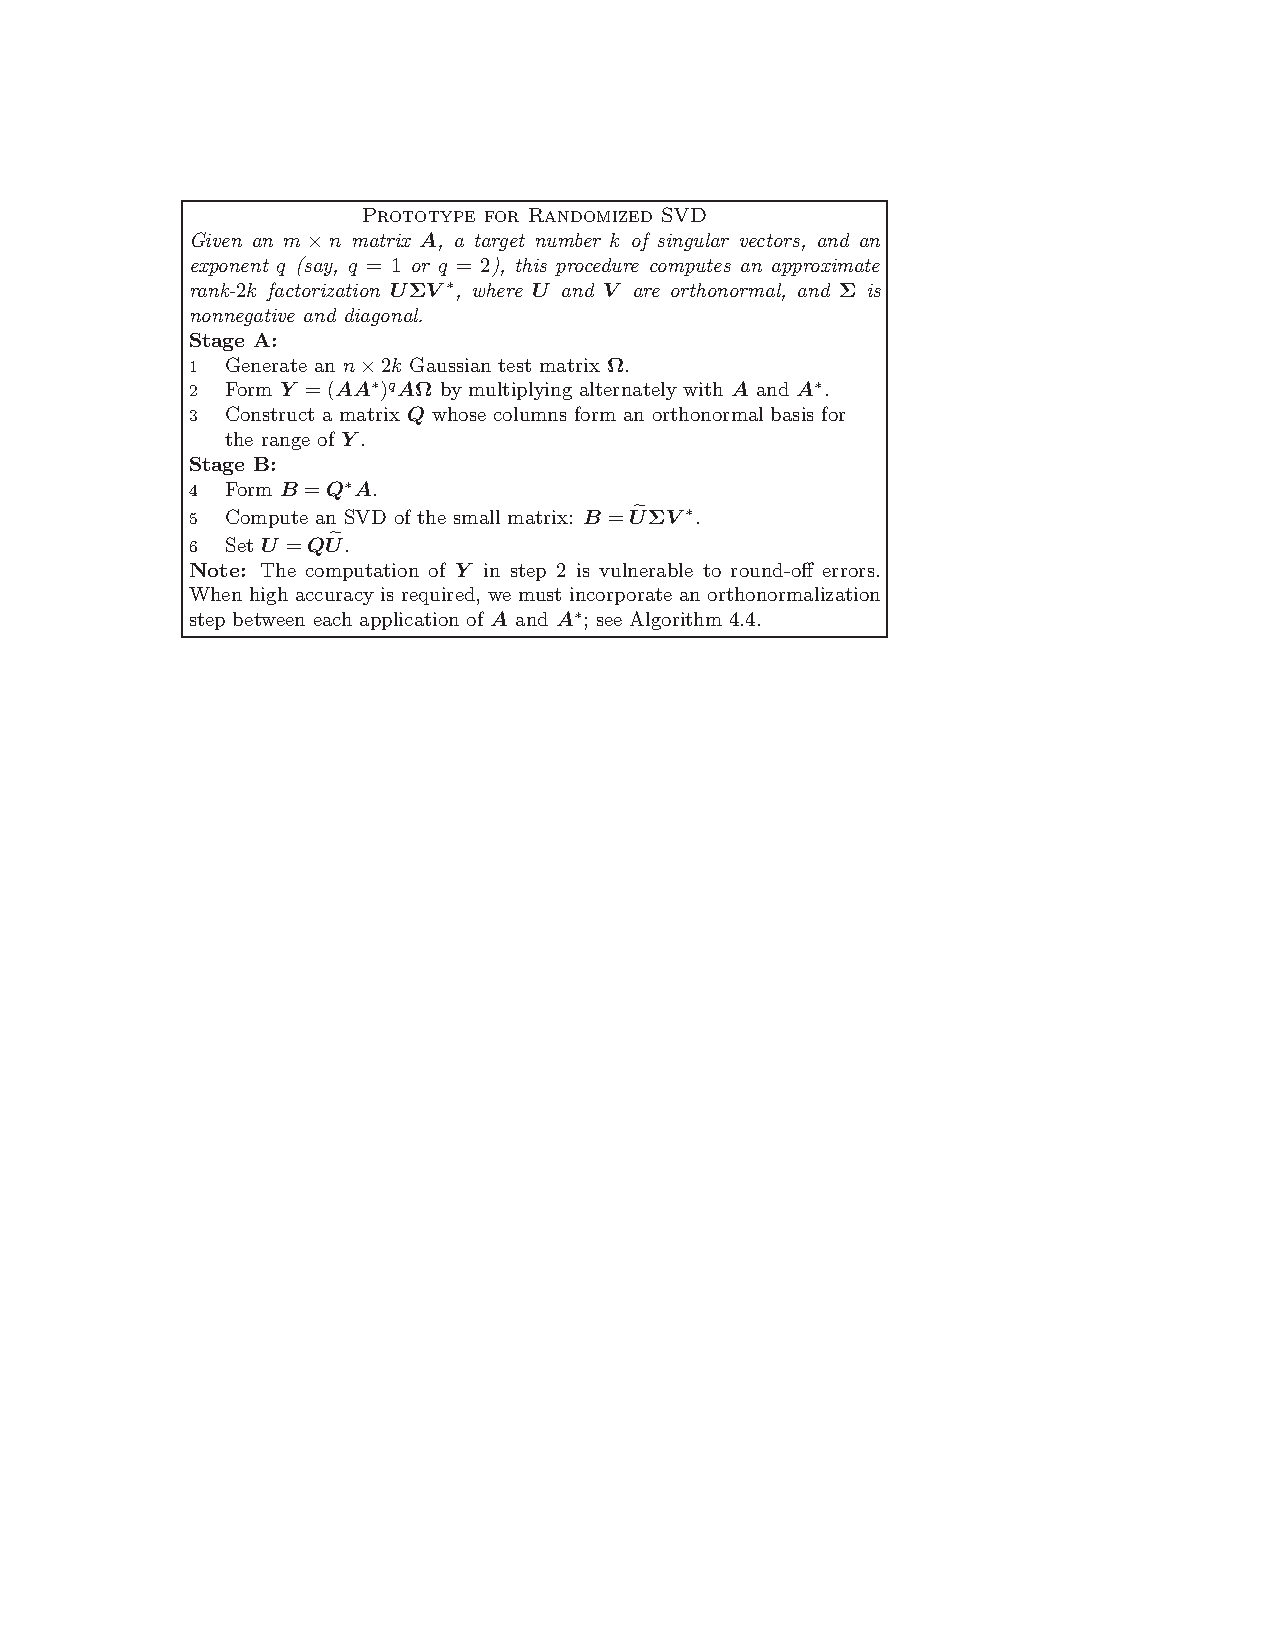
\includegraphics[height=.41\textheight]{../common/pics/randsvd/randSVDalg}
      \\
      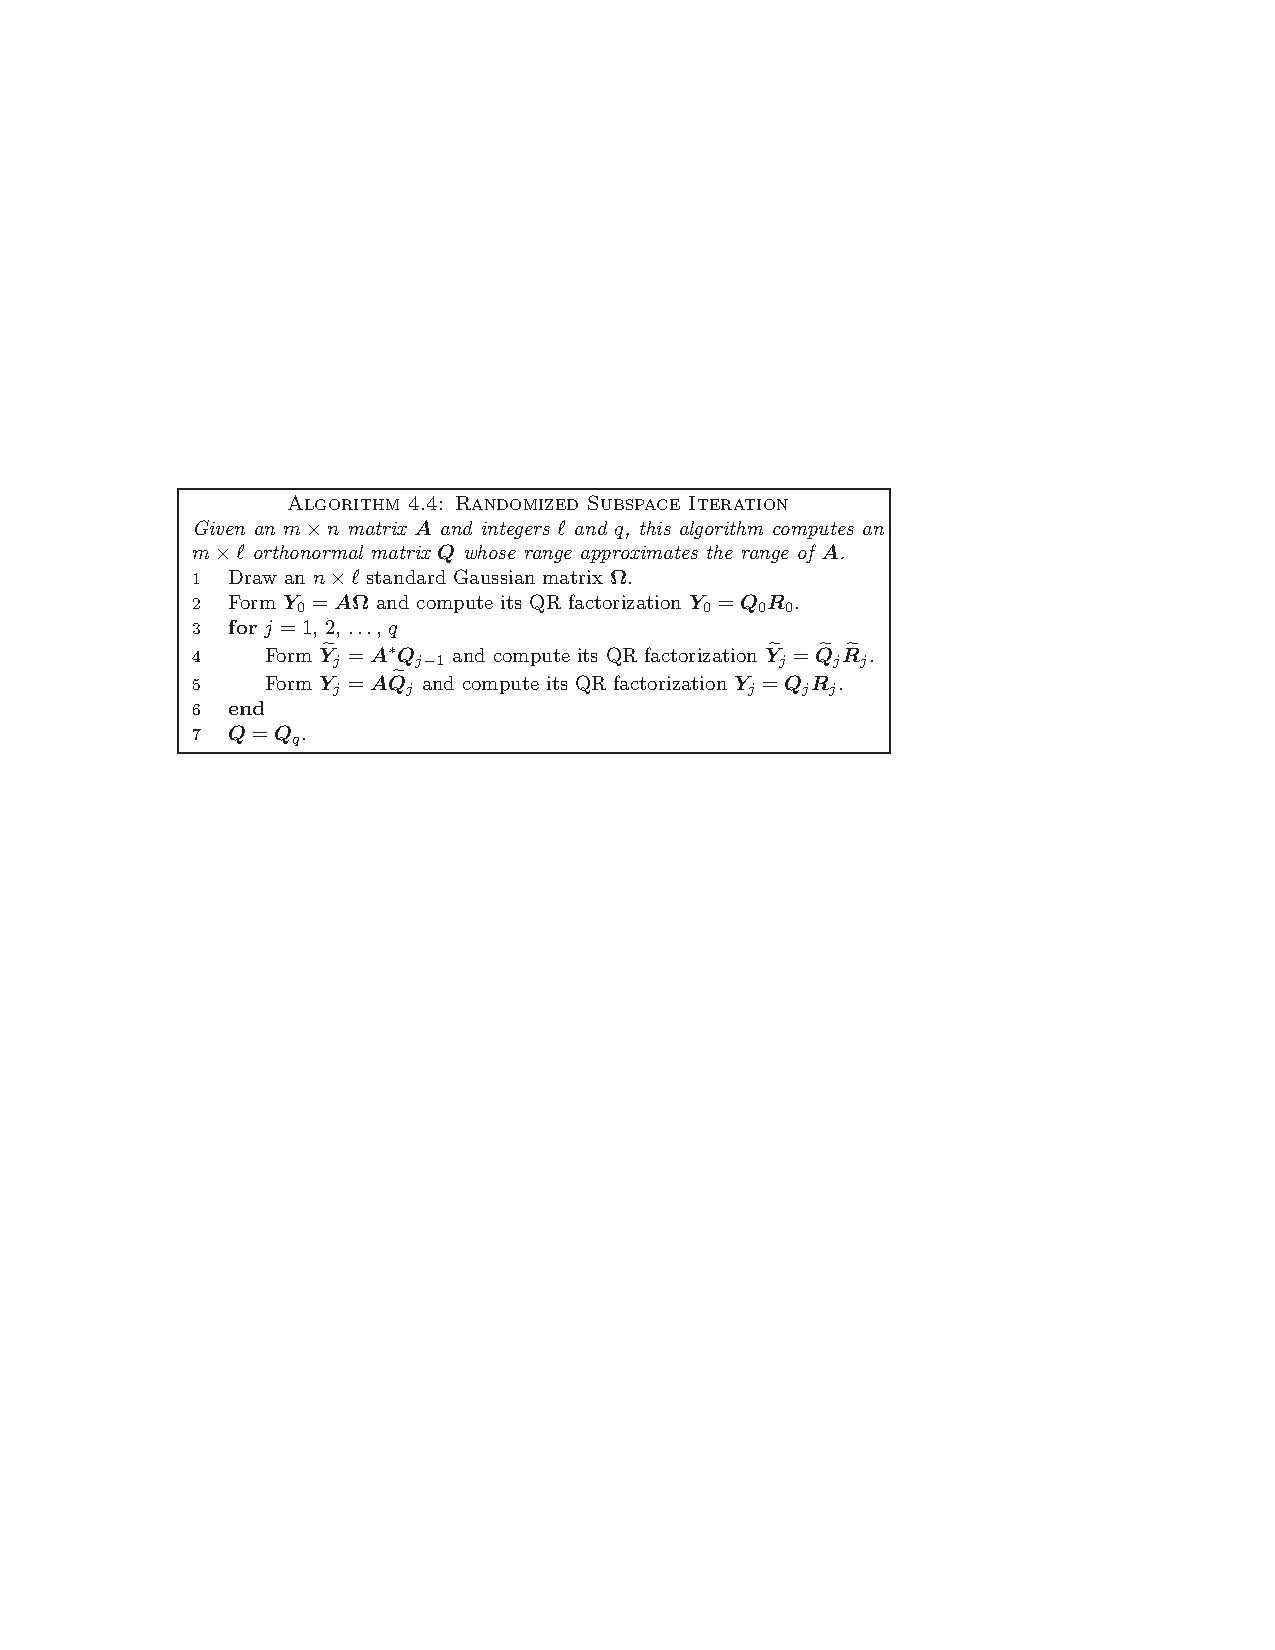
\includegraphics[height=.26\textheight]{../common/pics/randsvd/randSVDalg4_4}
    \end{center}
  \end{minipage}
%   \hspace{.01cm}
  \begin{minipage}{0.43\textwidth}
\begin{lstlisting}[title=Serial 
R,basicstyle=\tiny,backgroundcolor=\color{grayish} 
,numberstyle=\tiny\color{black},keywordstyle=\color{black},commentstyle=\color{ 
dkgreen},stringstyle=\color{black},escapeinside={(*@}{@*)}]
randSVD <- function(A, k, q=3)
  {
    ## Stage A
    Omega <- (*@ matrix(rnorm(n*2*k),@*)
      (*@ nrow=n, ncol=2*k) @*)
    Y <- A %*% Omega
    Q <- qr.Q(qr(Y))
    At <- t(A)
    for(i in 1:q)
      {
        Y <- At %*% Q
        Q <- qr.Q(qr(Y))
        Y <- A %*% Q
        Q <- qr.Q(qr(Y))
      }
    
    ## Stage B
    B <- t(Q) %*% A
    U <- La.svd(B)$u
    U <- Q %*% U
    U[, 1:k]
  }
\end{lstlisting} %balance$
\end{minipage}
{\fontsize{6pt}{10}\selectfont $^1$Halko, Martinsson, 
  and Tropp. 2011. Finding structure with randomness: probabilistic
  algorithms  for constructing \\[-1ex] approximate matrix decompositions
  \emph{SIAM Review} \textbf{53} 217--288}
\end{block}
\end{frame}


\begin{frame}[fragile]
 \fontsize{8pt}{10}\selectfont
\begin{block}{Randomized truncated SVD}
  \hfill
  \begin{minipage}{0.430\textwidth}
\begin{lstlisting}[title=Serial 
R,basicstyle=\tiny,backgroundcolor=\color{grayish} 
,numberstyle=\tiny\color{black},keywordstyle=\color{black},commentstyle=\color{ 
dkgreen},stringstyle=\color{black},escapeinside={(*@}{@*)}]
randSVD <- function(A, k, q=3)
  {
    ## Stage A
    Omega <- (*@ \textcolor{blue}{matrix(rnorm(n*2*k),} @*)
      (*@ \textcolor{blue}{ nrow=n, ncol=2*k)} @*)
    Y <- A %*% Omega
    Q <- qr.Q(qr(Y))
    At <- t(A)
    for(i in 1:q)
      {
        Y <- At %*% Q
        Q <- qr.Q(qr(Y))
        Y <- A %*% Q
        Q <- qr.Q(qr(Y))
      }
    
    ## Stage B
    B <- t(Q) %*% A
    U <- La.svd(B)$u
    U <- Q %*% U
    U[, 1:k]
  }
\end{lstlisting} %balance$
  \end{minipage}
  \hfill
  \begin{minipage}{0.430\textwidth}
\begin{lstlisting}[title=Parallel pbdR,basicstyle=\tiny,backgroundcolor=\color{
grayish}, numberstyle=\tiny\color{black},keywordstyle=\color{black},
commentstyle=\color{dkgreen},stringstyle=\color{black},escapeinside={(*@}{@*)}]
randSVD <- function(A, k, q=3)
  {
    ## Stage A
    Omega <- (*@ \textcolor{blue}{ddmatrix("rnorm",} @*)
      (*@ \textcolor{blue}{nrow=n, ncol=2*k)} @*)
    Y <- A %*% Omega
    Q <- qr.Q(qr(Y))
    At <- t(A)      
    for(i in 1:q)
      {
        Y <- At %*% Q   
        Q <- qr.Q(qr(Y))
        Y <- A %*% Q    
        Q <- qr.Q(qr(Y))
      }
    
    ## Stage B
    B <- t(Q) %*% A     
    U <- La.svd(B)$u 
    U <- Q %*% U     
    U[, 1:k]
  }
\end{lstlisting}  % balancing $
  \end{minipage}
\hfill
\end{block}
\end{frame}

\begin{frame}
  \begin{block}{From journal to scalable code and scaling data in one day.}
    \begin{center}
      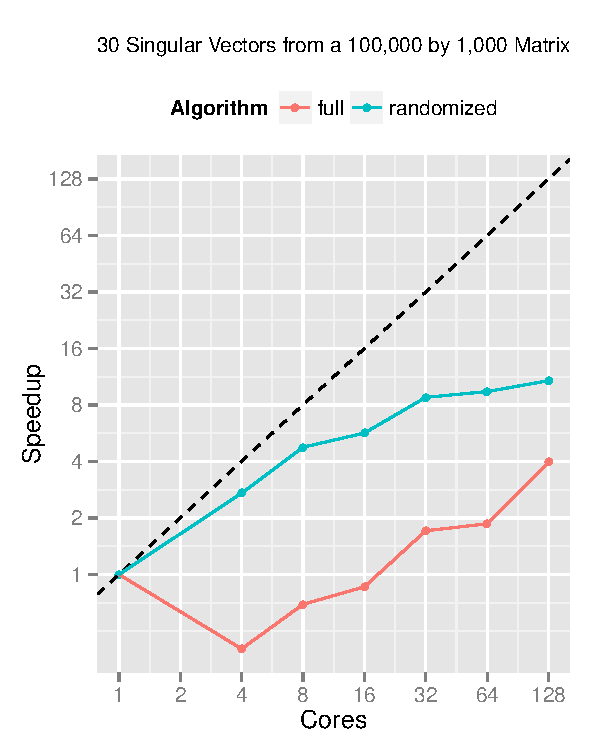
\includegraphics[width=.4\textwidth]{../common/pics/randsvd/randSVDspeedup}
      \hspace{1cm}
      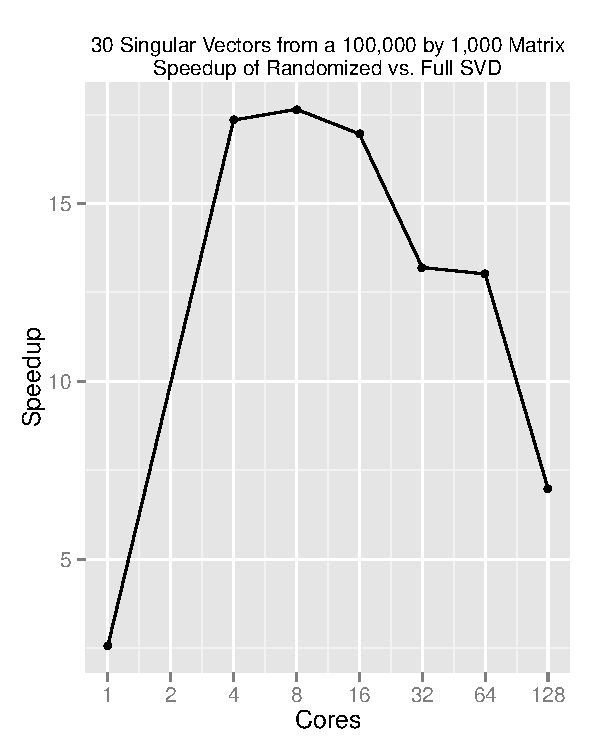
\includegraphics[width=.4\textwidth]{../common/pics/randsvd/randSpeedupSVD}
    \end{center}
  \end{block}
\end{frame}


